\documentclass{article}
\usepackage{amsmath}
\usepackage{amssymb}
\usepackage{graphicx}
\usepackage{hyperref}
\usepackage[version=4]{mhchem}


\begin{document}
In an acute triangle \(A B C, B E\) is the altitude and \(C F\) is the median. \(\angle A C F=30^{\circ}\). Which of the following is true about the relationship of \(B E\) and \(C F\) ?\\
\centering
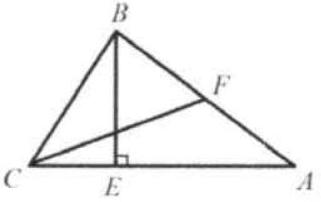
\includegraphics[width=\textwidth]{images/035.jpg}\\
(A) \(B E>C F\)\\
(B) \(B E=C F\)\\
(C) \(B E<C F\)\\
(D)

Solution: (B).\\
Take \(D\), the midpoint of \(A E\). Connect \(F D . F D / / B E\) is the midline of triangle \(A B E\), with \(F D \perp A C\).\\
Therefore, \(F D=\frac{1}{2} B E\).\\
In right triangle \(C D F\), since \(\angle A C F=30^{\circ}\), \(F D=\frac{1}{2} C F\).\\
\centering
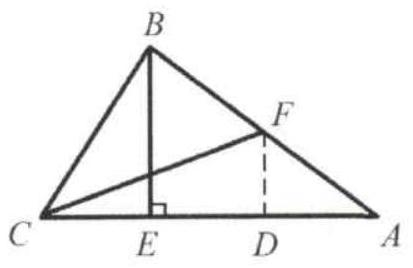
\includegraphics[width=\textwidth]{images/036(2).jpg}

Thus \(F D=\frac{1}{2} B E=\frac{1}{2} C F \quad \Rightarrow \quad B E=C F\).\\
The answer is (B).\\

\end{document}
